\section{Experimental Evaluation - Activity Forecasting}

\begin{frame}
	\frametitle{Evaluating an Activity Forecasting Method}
	
	\Large
	
	\vspace{0.45cm}
	
	The Negative Log-Loss (NLL) represents the expectation of the log-likelihood of a trajectory $ s $
	under a policy $ \pi(a \, | \, s) $:
	\vspace{-0.1cm}
	\begin{equation*}
		NLL(s) = E_{\pi(a \, | \, s)} \Big [ -\log \prod\nolimits_t \pi(a_t \, | \, s_t)  \Big ]
	\end{equation*}
	
	\vspace{0.1cm}
	
	This metric measures the probability of drawing the demonstrated trajectory from the learnt
	distribution over all possible trajectories. \\
\end{frame}

\begin{frame}
	\frametitle{Experimental Evaluation}
	\framesubtitle{Activity Forecasting}
	
	\large
	
	\vspace{-0.1cm}
	
	\begin{columns}[t]
		\only<1->
		{
			\column{0.9\textwidth}
			
			\begin{block}{Predicting Future Agent Motions}
				inferring agent goals accurately in a varied set of environments
			\end{block}
			
			\column{0.05\textwidth}
		}
	\end{columns}
	
	\vspace{0.1cm}
	
	\begin{center}
		\begin{tikzpicture}
			\node at (0,0) [draw=black,ultra thick,inner sep=0pt]  {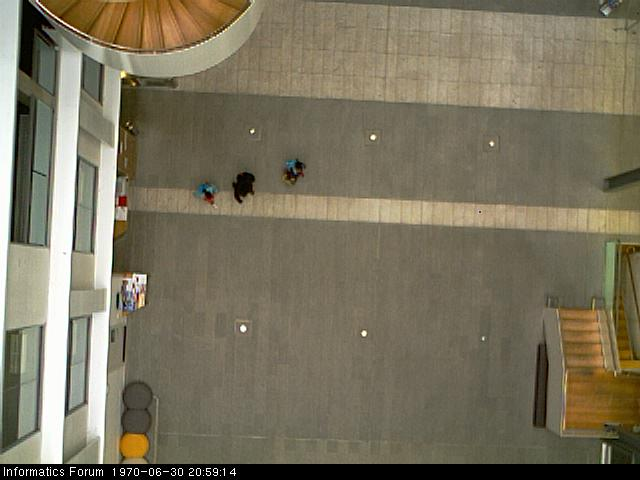
\includegraphics[height=2.9cm]{Figures/InformaticsForum}};
			\node at (4,0) [draw=black,ultra thick,inner sep=0pt]  {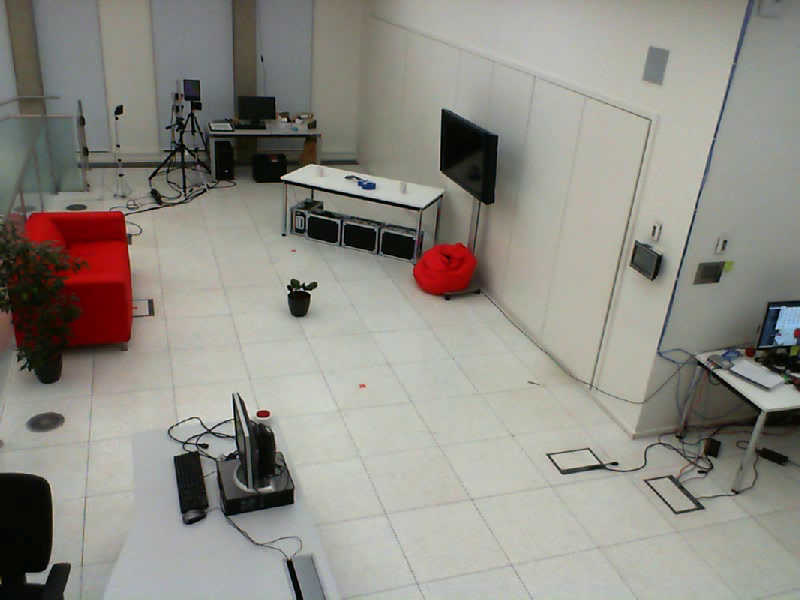
\includegraphics[height=2.9cm]{Figures/InSpace_FrontCamera}};
			\node at (7.98,0) [draw=black,ultra thick,inner sep=0pt]  {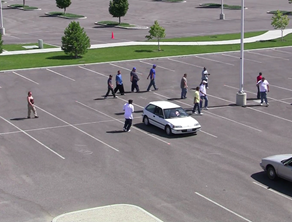
\includegraphics[height=2.9cm]{Figures/VIRAT}};
		\end{tikzpicture}
	\end{center}
	
	\vspace{0.15cm}
	
	\tiny
	
	\textbf{IRL-based Prediction of Goals for Dynamic Environments}\\
	F. Previtali, A. Bordallo, S. Ramamoorthy \\
	\emph{Workshop on Machine Learning for Social Robotics at ICRA, 2015} \\
	
	\vspace{0.1cm}
	
	\textbf{Predicting Future Agent Motions for Dynamic Environments}\\
	F. Previtali, A. Bordallo, L. Iocchi, S. Ramamoorthy \\
	\emph{International Conference on Intelligent Robots and Systems} [submitted] \\
\end{frame}

\begin{frame}
	\frametitle{Quantitative Evaluation}
	\framesubtitle{Activity Forecasting}
	
	\begin{figure}
		\centering
		\begin{tikzpicture}
			\node at (0,0) [draw=white,ultra thick,inner sep=0pt]
			{
				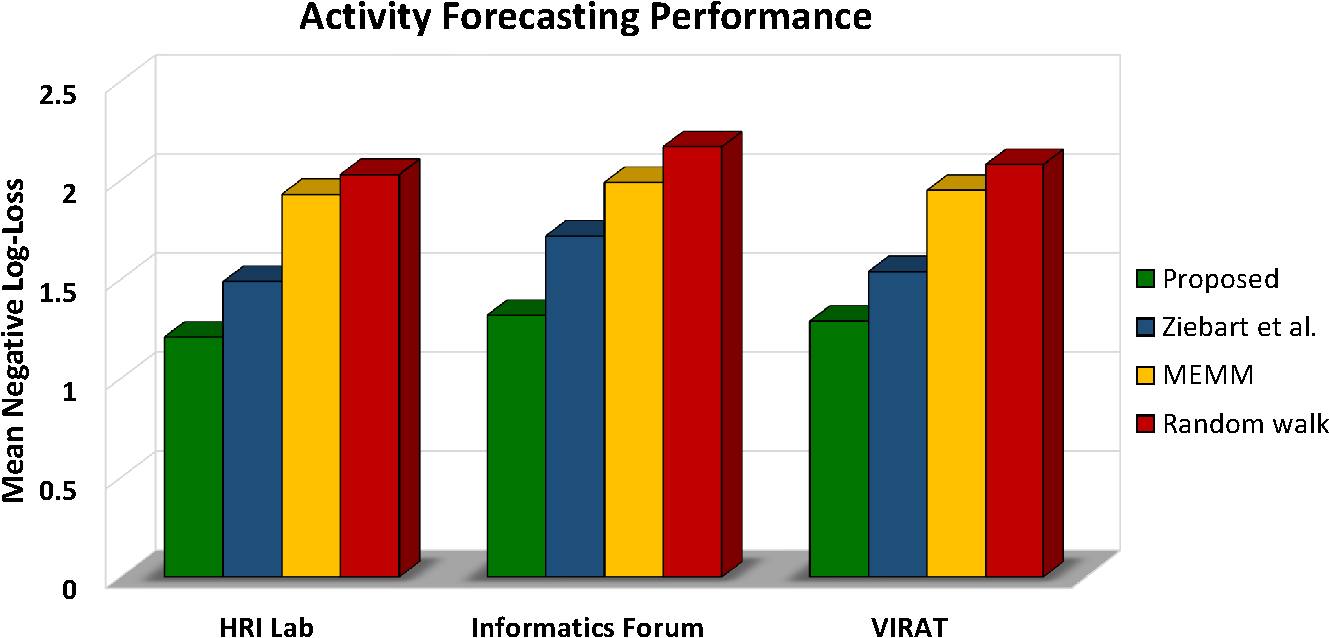
\includegraphics[width=\linewidth]{Figures/QuantitativeEvaluation}
			};
		\end{tikzpicture}
	\end{figure}
\end{frame}

%\begin{frame}
%	\frametitle{Qualitative Evaluation}
%	\framesubtitle{InSpace}
%	
%	\begin{figure}[!h]
%		\centering
%		\includemovie[inline=false,text=
%		{
%			\begin{tikzpicture}
%				\node at (0,0) [draw=black,ultra thick,inner sep=0pt]
%				{
%					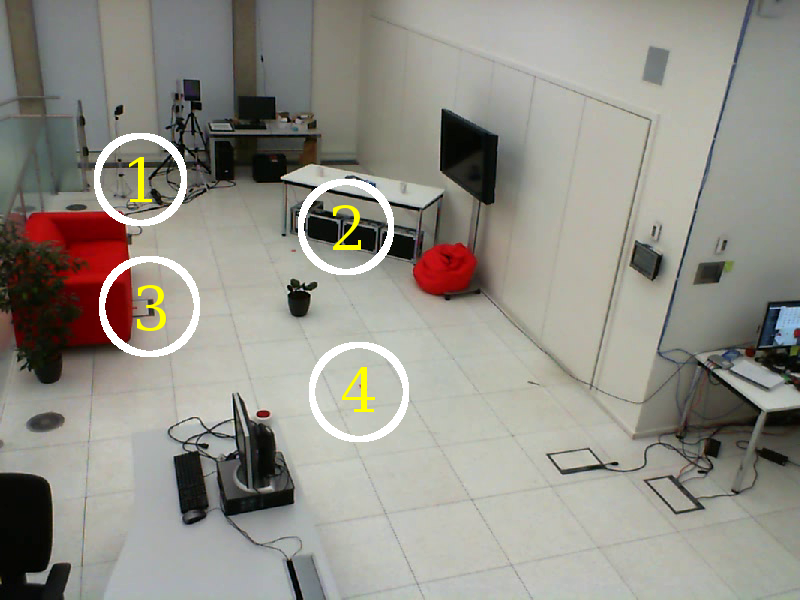
\includegraphics[width=0.65\linewidth]{Figures/InSpace_FrontCamera_Goals}
%				};
%			\end{tikzpicture}
%		}]{}{}{../Videos/5-ActivityForecasting/PTracking-House.avi}
%	\end{figure}
%\end{frame}

\begin{frame}
	\frametitle{Experimental Evaluation}
	\framesubtitle{Context-Aware Navigation}
	
	\vspace{0.05cm}
	
	\begin{center}
		\begin{tikzpicture}
			\node at (0,0) [draw=black,ultra thick,inner sep=0pt]
			{
				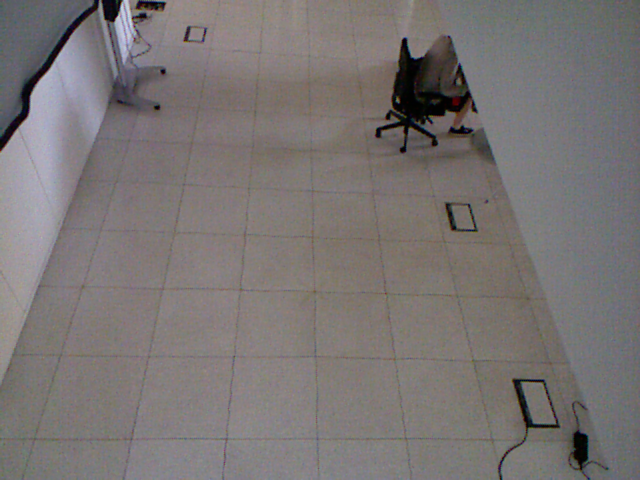
\includegraphics[height=2.6cm]{Figures/Kinect-1}
			};
			\node at (3.62,0) [draw=black,ultra thick,inner sep=0pt]
			{
				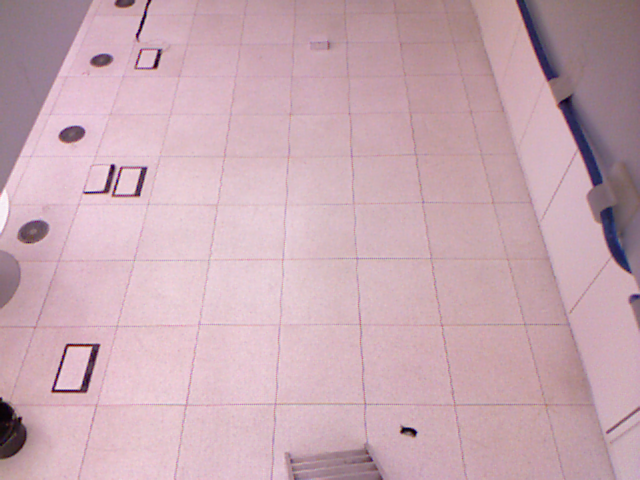
\includegraphics[height=2.6cm]{Figures/Kinect-2}
			};
			\node at (7.24,0) [draw=black,ultra thick,inner sep=0pt]
			{
				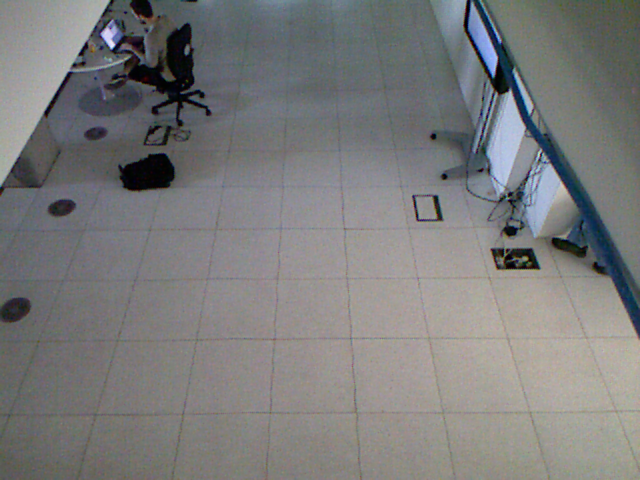
\includegraphics[height=2.6cm]{Figures/Kinect-3}
			};
		\end{tikzpicture}
	\end{center}
	
	\vspace{-0.4cm}
	\tiny
	
	\begin{tabbing}
		\hspace{1.5cm}
		\textbf{Counterfactual Reasoning about Intent for Interactive Navigation in Dynamic
				Environments} \\
		\hspace{1.5cm}
		A. Bordallo, F. Previtali, N. Nardelli, S. Ramamoorthy \\
		\hspace{1.5cm}
		\emph{IEEE/RSJ International Conference on Intelligent Robots and Systems, 2015} \\
	\end{tabbing}
	
	\vspace{-0.55cm}
	
	\begin{center}
		\begin{tikzpicture}
			\node at (0,0) [draw=black,ultra thick,inner sep=0pt]
			{
				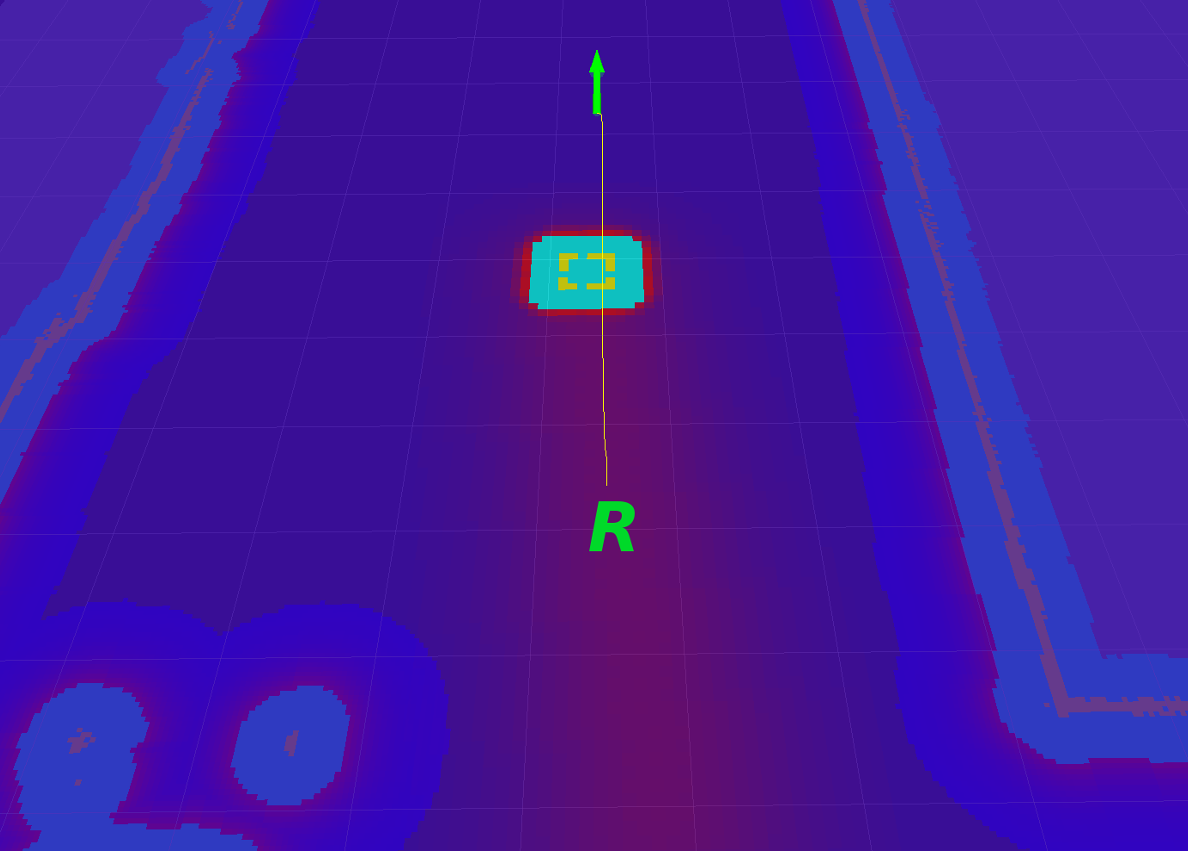
\includegraphics[height=2.35cm]{Figures/ConstantVelocityComparison}
			};
			\node at (3.45,0) [draw=black,ultra thick,inner sep=0pt]
			{
				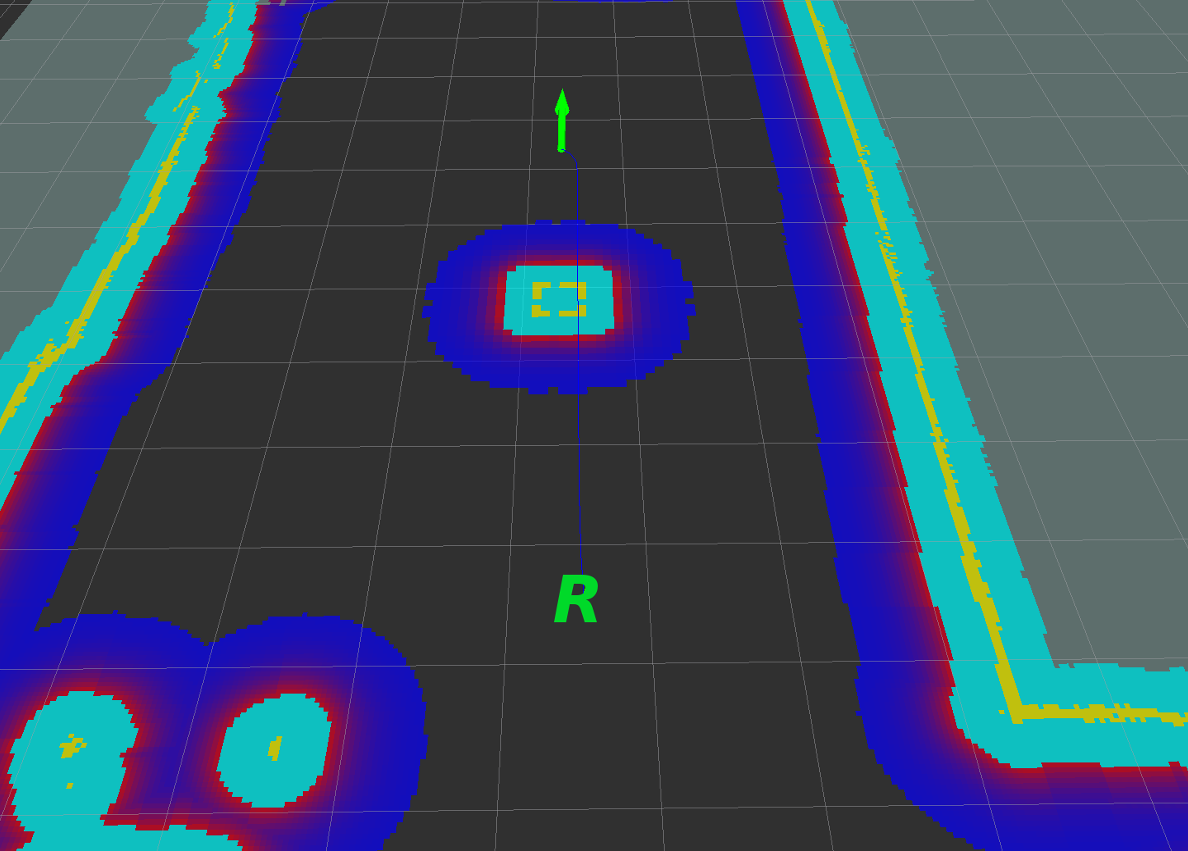
\includegraphics[height=2.35cm]{Figures/ProxemicsComparison}
			};
			\node at (6.9,0) [draw=black,ultra thick,inner sep=0pt]
			{
				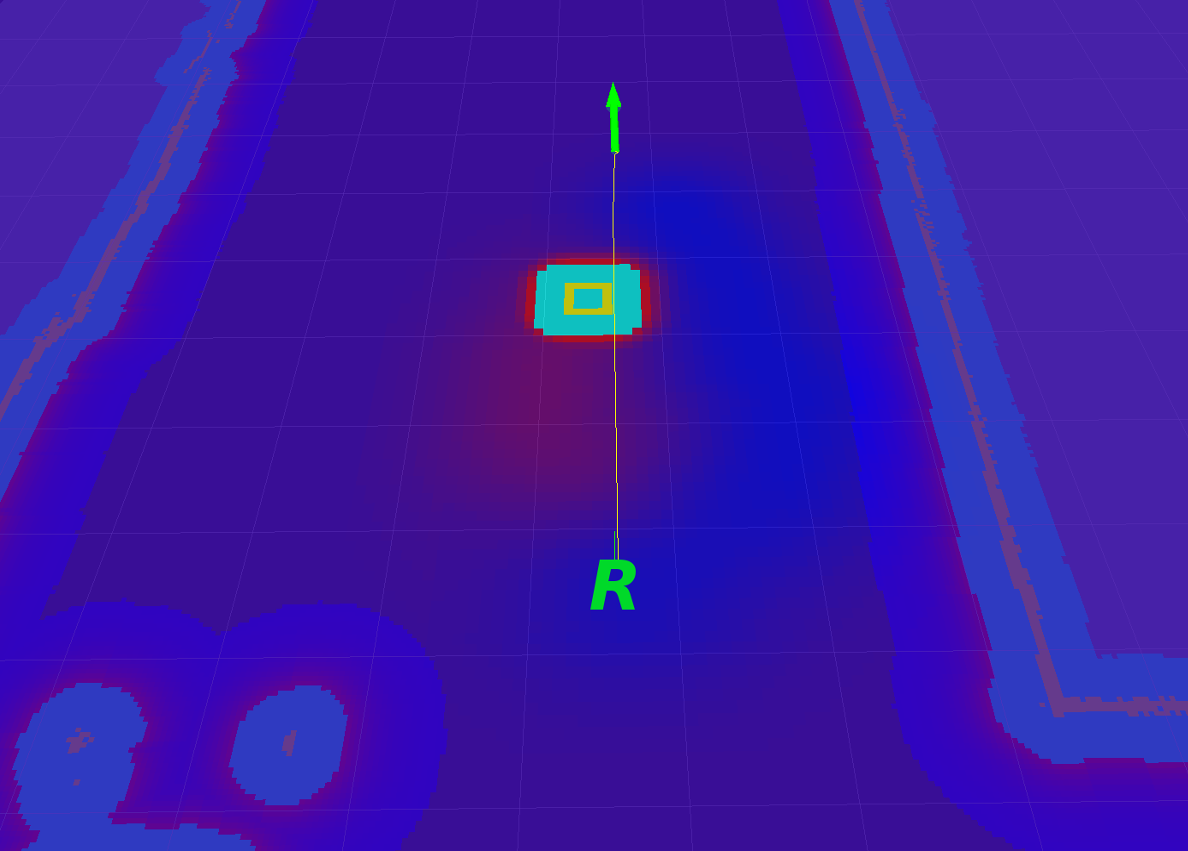
\includegraphics[height=2.35cm]{Figures/InteractiveCostmapComparison}
			};
		\end{tikzpicture}
	\end{center}
	
	\vspace{-0.4cm}
	
	\begin{tabbing}
		\hspace{1.55cm}
		\textbf{Interactive Costmaps: Integrating Prediction and Planning with Counterfactual
				Reasoning} \\
		\hspace{1.55cm}
		A. Bordallo, F. Previtali, S. Ramamoorthy \\
		\hspace{1.55cm}
		\emph{IEEE/RSJ International Conference on Intelligent Robots and Systems} [submitted] \\
	\end{tabbing}
\end{frame}

\begin{frame}
	\frametitle{Qualitative Evaluation}
	\framesubtitle{InSpace}
	
	\begin{figure}[!h]
		\centering
		\includemovie[inline=false,text=
		{
			\begin{tikzpicture}
				\node at (0,0) [draw=black,ultra thick,inner sep=0pt]
				{
					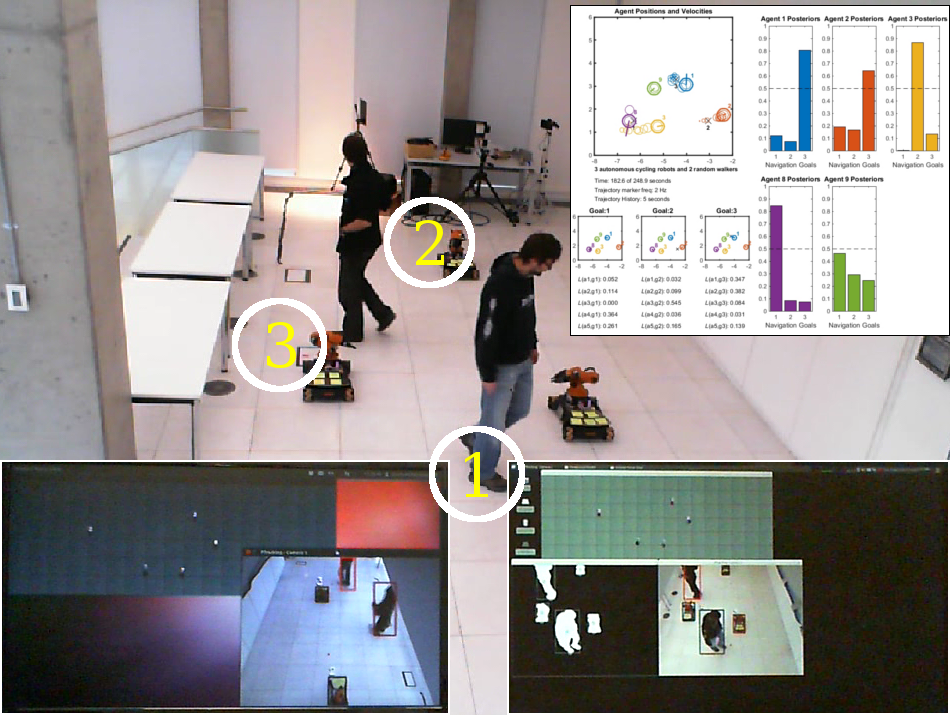
\includegraphics[width=0.65\linewidth]{Figures/InSpace}
				};
			\end{tikzpicture}
		}]{}{}{../Videos/3-Youbot/PTracking-2People_3PlanningYoubots.mpg}
	\end{figure}
\end{frame}

%\begin{frame}
%	\frametitle{Experimental Evaluation}
%	\framesubtitle{Interactive Costmaps}
%	
%	\large
%	
%	\begin{columns}[t]
%		\only<1->
%		{
%			\column{0.8\textwidth}
%			
%			\begin{block}{Effective Social Motion Planning}
%				reasoning about interactive agents' intention in the environment in order to adapt the
%				costmap over time
%			\end{block}
%			
%			\column{0.15\textwidth}
%		}
%	\end{columns}
%	
%	\vspace{0.2cm}
%	
%	\begin{center}
%		\begin{tikzpicture}
%			\node at (0,0) [draw=black,ultra thick,inner sep=0pt]  {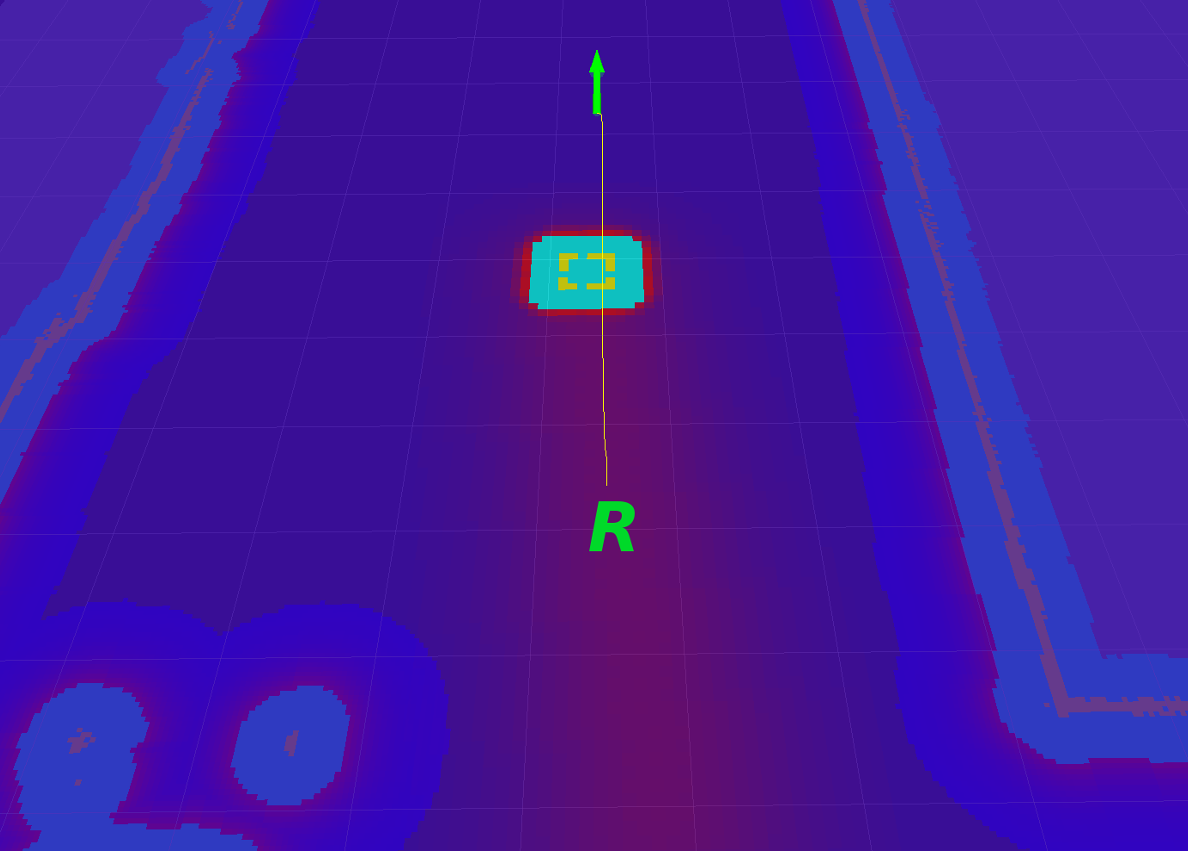
\includegraphics[height=2.8cm]{Figures/ConstantVelocityComparison}};
%			\node at (4.05,0) [draw=black,ultra thick,inner sep=0pt]  {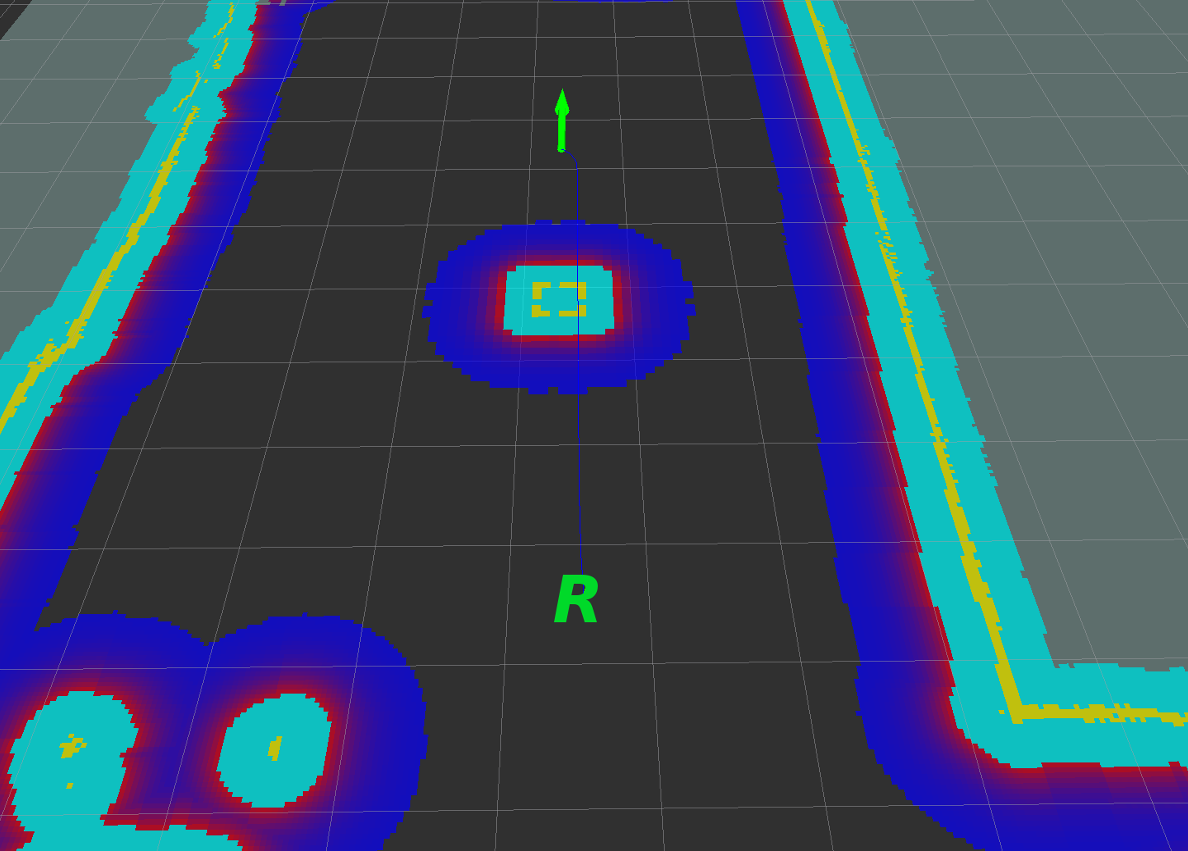
\includegraphics[height=2.8cm]{Figures/ProxemicsComparison}};
%			\node at (8.11,0) [draw=black,ultra thick,inner sep=0pt]  {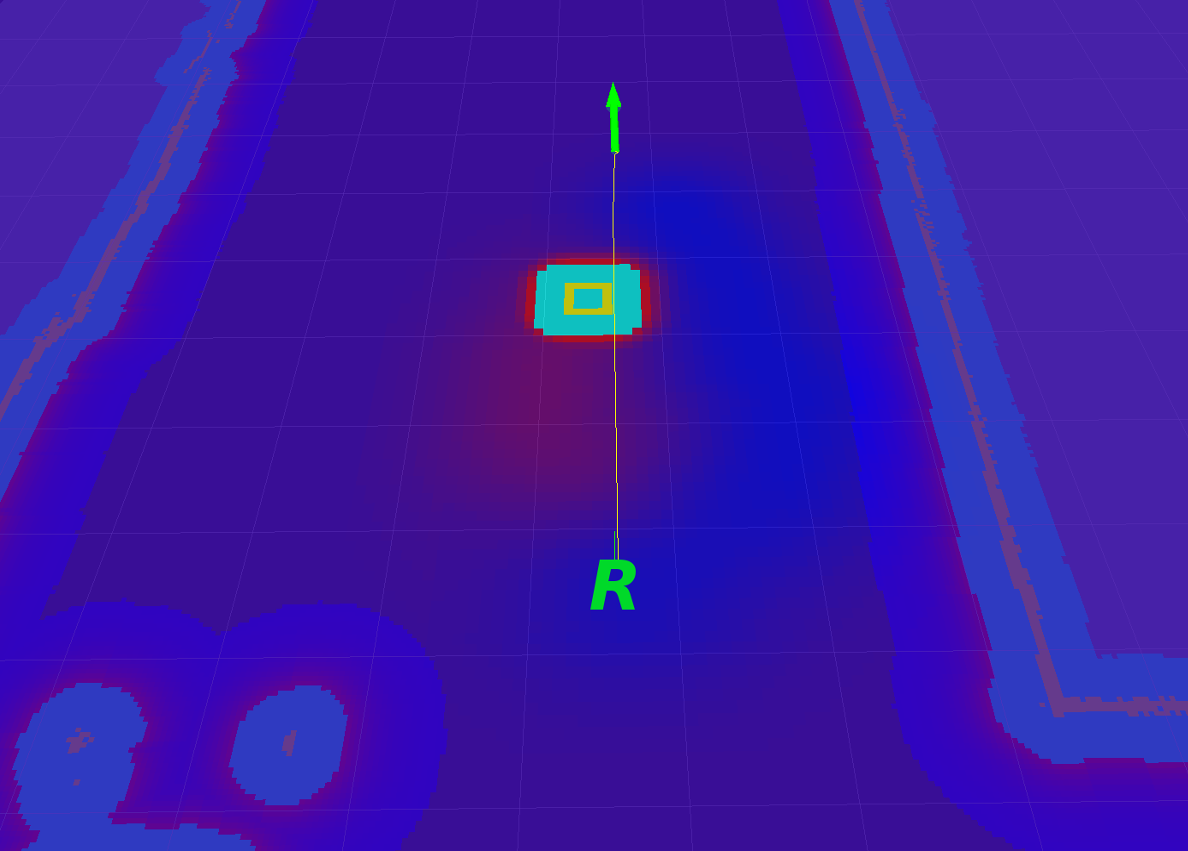
\includegraphics[height=2.8cm]{Figures/InteractiveCostmapComparison}};
%		\end{tikzpicture}
%	\end{center}
%	
%	\vspace{0.36cm}
%	
%	\tiny
%	
%	\textbf{Interactive Costmaps: Integrating Prediction and Planning with Counterfactual Reasoning}\\
%	A. Bordallo, F. Previtali, S. Ramamoorthy \\
%	\emph{IEEE/RSJ International Conference on Intelligent Robots and Systems, 2015} [submitted] \\
%\end{frame}
%
%\begin{frame}
%	\frametitle{Quantitative Evaluation}
%	\framesubtitle{InSpace}
%	
%	\begin{table}
%		\centering
%		\caption{Comparison of costmap experiments, obstacle layer is used as a baseline. CPU\% shows
%				 average measured consumption and p.a. shows additional load per agent. Execution time
%				 shows time required for costmap generation. Experiment times show average/worst time
%				 over all trials, where $\infty s$ denotes a timeout.}
%		\def\arraystretch{1.3}
%		\vspace{-0.3cm}
%		\resizebox{\textwidth}{!}
%		{
%			\begin{tabular}{lcccccc}
%				Method & CPU & Execution Time & Passing Time & Crossing Time & Collisions &
%				Near-collision \\ \hline
%				Obstacle layer (Baseline) & -\% & -s & 5/$\infty$s & 5/$\infty$s & 80\% & 70\% \\
%				Constant Velocity model & 4\%+1\% p.a. & 5ms p.a. & 15/20s & 12/18s & 40\% & 60\% \\
%				Proxemics and social & 3\%+2\% p.a. & 5ms + 5ms p.a. & 8/28s & 12/14s & 20\% & 50\% \\
%				\textbf{Interactive Costmap} & \textbf{6\%+2\% p.a.} & \textbf{5ms + 5ms p.a.} &
%				\textbf{7/8s} & \textbf{8/9s} & \textbf{10\%} &  \textbf{20\%}  \\
%			\end{tabular}
%		}
%	\end{table}
%\end{frame}
%
%\begin{frame}
%	\frametitle{Qualitative Evaluation}
%	\framesubtitle{InSpace}
%	
%	\begin{figure}[!h]
%		\centering
%		\includemovie[inline=false,text=
%		{
%			\begin{tikzpicture}
%				\node at (0,0) [draw=black,ultra thick,inner sep=0pt]
%				{
%					\includegraphics[width=0.65\linewidth]{Figures/InteractiveCostmap}
%				};
%			\end{tikzpicture}
%		}]{}{}{../Videos/3-Youbot/InteractiveCostmaps.avi}
%	\end{figure}
%\end{frame}
